%-----------------------------------------------------------------
\chapter{Introduzione}
\label{ch:intro}
%-----------------------------------------------------------------

\flex\ � una scheda dedicata che pu� essere utilizzata da tutti gli
sviluppatori di sistemi embedded che vogliono sfruttare a pieno le
potenzialit� dei microcontrollori \dspic\ prodotti da Microchip.

\flex\ � nata come una scheda di sviluppo che pu� essere utilizzata
per sviluppare e verificare applicazioni dedicate e real-time per i
microcontrollori Microchip. Le caratteristiche principali del sistema
sono:

\begin{itemize}
\item un design particolarmente robusto dal punto di vista elettronico
  (in particolare, \flex\ Full include un alimentatore switching);
\item architettura modulare (realizzata utilizzando delle schede
  figlie, dette anche ``daughter boards'');
\item la disponibilit� di un crescente numero di applicazioni di esempio;
\item il supporto completo da parte del kernel real-time \ee\ prodotto
  da Evidence Srl;
\item la disponibilit� di un generatore di codice capace di generare
  applicazioni finite a partire da design basati su Scilab/Scicos.
\end{itemize}

Il design compatto ed essenziale della scheda \flex\ permette il suo
utilizzo non solo per sperimentazioni ma anche per prodotti industriali
come ad esempio:
\begin{itemize}
\item Convertitori di protocollo;
\item Web server minimali;
\item Sistemi di acquisizione;
\item Sistemi wireless;
\item Sistemi di controllo digitale.
\end{itemize}



%-----------------------------------------------------------------
\chapter{I produttori della scheda \flex}
\label{ch:partnership}
%-----------------------------------------------------------------

\begin{center}
\begin{minipage}{4.5cm}
  %
\includegraphics[width=4cm]{../common/LogoEvidence.eps}
  
\includegraphics[width=4cm, bb=0 0 417 194]{../common/LogoEvidence.png}
\end{minipage}
\begin{minipage}{4.5cm}
  
\includegraphics[width=4cm]{../common/LogoES.eps}
\end{minipage}\\
\end{center}

La piattaforma \flex\ � il risultato della collaborazione di due
aziende italiane che lavorano nell'ambito dei sistemi embedded:
Evidence Srl ed Embedded Solutions Srl.

Le due aziende hanno unito le loro capacit�, rispettivamente nel campo
dei sistemi operativi real-time e nello sviluppo di sistemi HW
dedicati, per creare una soluzione completa, semplice da utilizzare e
compatta per creare applicazioni utilizzando i microcontrollori
\dspic\ di Microchip.

In particolare, 
\begin{itemize}
\item Evidence Srl ha contribuito fornendo una versione GPL del kernel
  real-time \ee, assieme ad un insieme di applicazioni di esempio che
  utilizzano la scheda \flex.
\item Embedded Solutions Srl ha fornito il design hardware, ed �
  responsabile della produzione delle schede \flex.
\end{itemize}

Oltre alla disponibilit� di una serie di schede figlie (``daughter
boards''), sono possibili personalizzazioni delle schede \flex. Per
maggiori informazioni, fare riferimento al Capitolo
\ref{ch:customizations}.



%-----------------------------------------------------------------
\chapter{Architettura}
\label{ch:arch}
%-----------------------------------------------------------------

L'architettura modulare fornita da \flex\ permette di integrare un
insieme di caratteristiche interessanti all'interno di una singola
scheda.

La configurazione di base di un sistema \flex\ � composto dalla sola
scheda di base. Le schede base di \flex\ ospitano un microcontrollore
\dspic\ di Microchip, e quasi tutti i pin del microcontrollore sono
esportati sugli appositi connettori. Gli utenti di Flex possono
collegare vari componenti elettronici in modo semplice ai pin del
microcontrollore per creare una applicazione specifica.

\begin{figure}[htb]
\begin{center}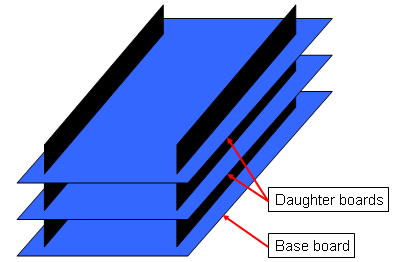
\includegraphics[
  width=12cm, bb=0 0 394 262]{images/piggyback.png}\end{center}
\caption{Architettura delle schede figlie \flex.}
\label{fig:piggyback}
\end{figure}

Come mostrato in Figura \ref{fig:piggyback}, varie schede figlie
possono essee collegate fisicamente una sopra l'altra alla scheda base
\flex. Le schede figlie offrono varie caratteristiche che possono
essere combinate in modo semplice per ottenere device complessi.

Evidence S.r.l. and Embedded Solutions S.r.l. forniscono un crescente
numero di schede figlie per svariate tipologie di applicazioni che
vanno dall'acquisizione di dati, al controllo digitale, alla
visualizzazione ed alla connessione di rete.


%-----------------------------------------------------------------
\section{Schede \flex\ base}
\label{sec:base_board}
%-----------------------------------------------------------------

Le schede base \flex\ sono state progettata esplicitamente per
limitare i vincoli dati allo sviluppatore che ha intenzione di
utilizzare i pin disponibili sul microcontrollore. Per questo motivo,
praticamente tutti i pin del microcontrollore sono stati riportati su
di un connettore a passo 2.54 mm, per semplificare lo sviluppo ``in
casa'' di schede figlie personalizzate.

Le schede base \flex\ possono ospitare il microcontrollore \dspic\ in
due modi diversi: il primo consiste nel fornire il microcontrollore
saldato direttamente sulla scheda, mentre il secondo prevede
l'utilizzo di uno zoccolo compatibile con i Plug-in Modules (PIM)
forniti da Microchip. La disponibilit� del montaggio di un PIM
permette allo sviluppatore di superare il limite massimo del numero di
scritture in flash dei microcontrollori \dspic. In particolare, una
volta raggiunto il limite di programmazione del microcontrollore �
possibile rimpiazzare il PIM.

La scheda base \flex\ � disponibile in due versioni:

\begin{itemize}
\item Versione Full, descritta nella Sezione \ref{sec:base-full};
\item Versione Light, descritta nella Sezione \ref{sec:base-light}.
\end{itemize}

\begin{figure}[htb]
\begin{center}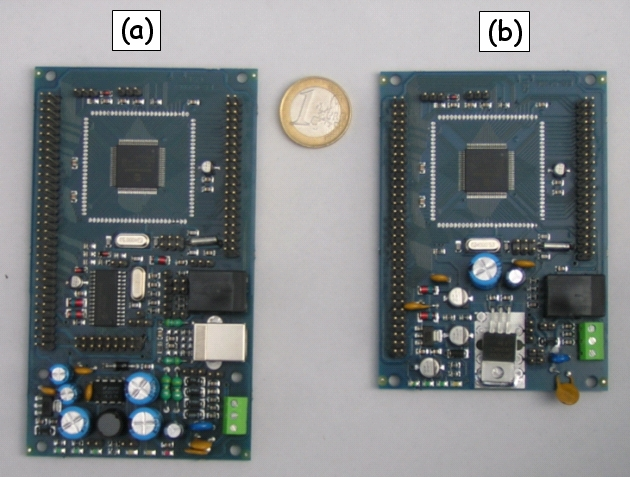
\includegraphics[
  width=12cm, bb=0 0 630 477]{images/flex_boards.jpg}\end{center}
\caption{Le schede base di \flex\ in versione Full (a) e Light (b).}
\label{fig:flex-boards}
\end{figure}

I connettori delle due versioni Full e Light delle schede base sono
compatibili, in modo tale che una scheda figlia e la relativa
applicazione sviluppate per la scheda base versione Full possono
essere facilmente spostate verso la scheda base versione Light e
viceversa.

%-----------------------------------------------------------------
\subsection{Scheda base: versione Full}
\label{sec:base-full}
%-----------------------------------------------------------------

La scheda base \flex\ in versione Full, visualizzata in Figura
\ref{fig:flex-full}, integra un alimentatore switching robusto che
permette l'uso di svariate sorgenti di alimentazione. Esso accetta
voltaggi in ingresso nel range 9 - 36 V. Il segnale di alimentazione �
poi filtrato ed adattato per generare i livelli di tensione interni a
3,3 e 5 V.

Inoltre, la scheda base \flex\ in versione Full include in modo nativo
una porta USB che pu� essere utilizata per il trasferimento dei dati
da e verso la scheda e, cosa pi� importante, come una interfaccia di
programmazione per il microcontrollore \dspic. La scheda Full �
disponibile opzionalmente con un programmatore compatibile con
Microchip ICD2 (ospitato sul microcontrollore PIC18 a bordo), che
permette di avere un sistema entrocontenuto che include sia la parte
di In Circuit Debugging che il microcontrollore senza la necessit� di
acquistare un debuggero o un programmatore a parte.

\begin{figure}[htb]
\begin{center}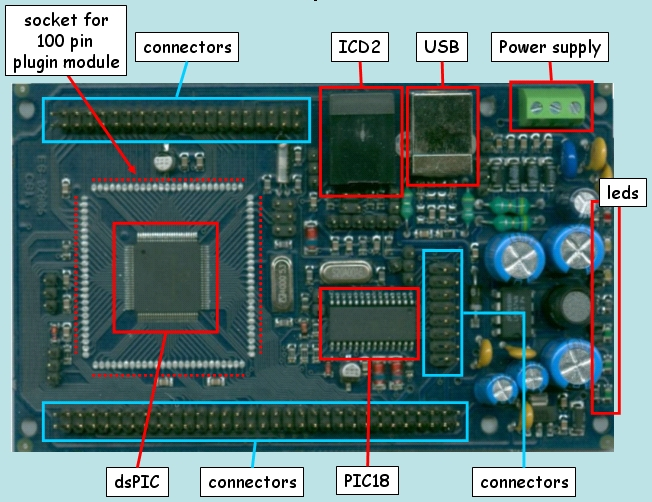
\includegraphics[
  width=12cm, bb=0 0 652 502]{images/flex_base_full.jpg}\end{center}
\caption{La scheda base \flex\ in versione Full.}
\label{fig:flex-full}
\end{figure}

I principali componenti della scheda base \flex\ versione Full,
visualizzata in Figura \ref{fig:flex-full}, sono:

\begin{itemize}
\item il microcontrollore Microchip \dspic;
\item lo zoccolo (quando presente) che ospita il Plug-In-Module (PIM)
  di Microchip;
\item il connettore per il debugger ICD2;
\item il connettore USB per la programmazione diretta del device;
\item i connettori di alimentazione;
\item un insieme di led per il monitraggio del funzionamento della scheda;
\item il microcontrollore Microchip PIC18 utilizzato per la
  programmazione integrata del dispositivo;
\item l'insieme dei connettori per le schede figlie (notare che la
  scheda in versione Full ha un connettore aggiuntivo per esportare i
  principali pin del PIC18).
\end{itemize}

I led disponibili sulla scheda sono elencati nella Tabella \ref{tab:leds-full}.

\begin{table}
\begin{centering}\begin{tabular}{|l|l|l|}
\hline 
Led & Colore & Funzione \tabularnewline
\hline \hline 
DL1 & verde & Alimentazione in ingresso \tabularnewline
\hline
DL2 & verde & Attivit� dell'alimentazione interna +5V \tabularnewline
\hline
DL3 & verde & Attivit� dell'alimentazione interna +3V \tabularnewline
\hline
DL4 & giallo & Led controllaro dal microcontrollore \dspic \tabularnewline
\hline
DL5 & giallo & Led controllato dal microcontrollore PIC18 \tabularnewline
\hline
DL6 & rosso & Monitor della connessione USB \tabularnewline
\hline 
\end{tabular}\par\end{centering}
\caption{Led disponibili sulla scheda base \flex\ versione Full.}
\label{tab:leds-full}
\end{table}


\begin{figure}[htb]
\begin{center}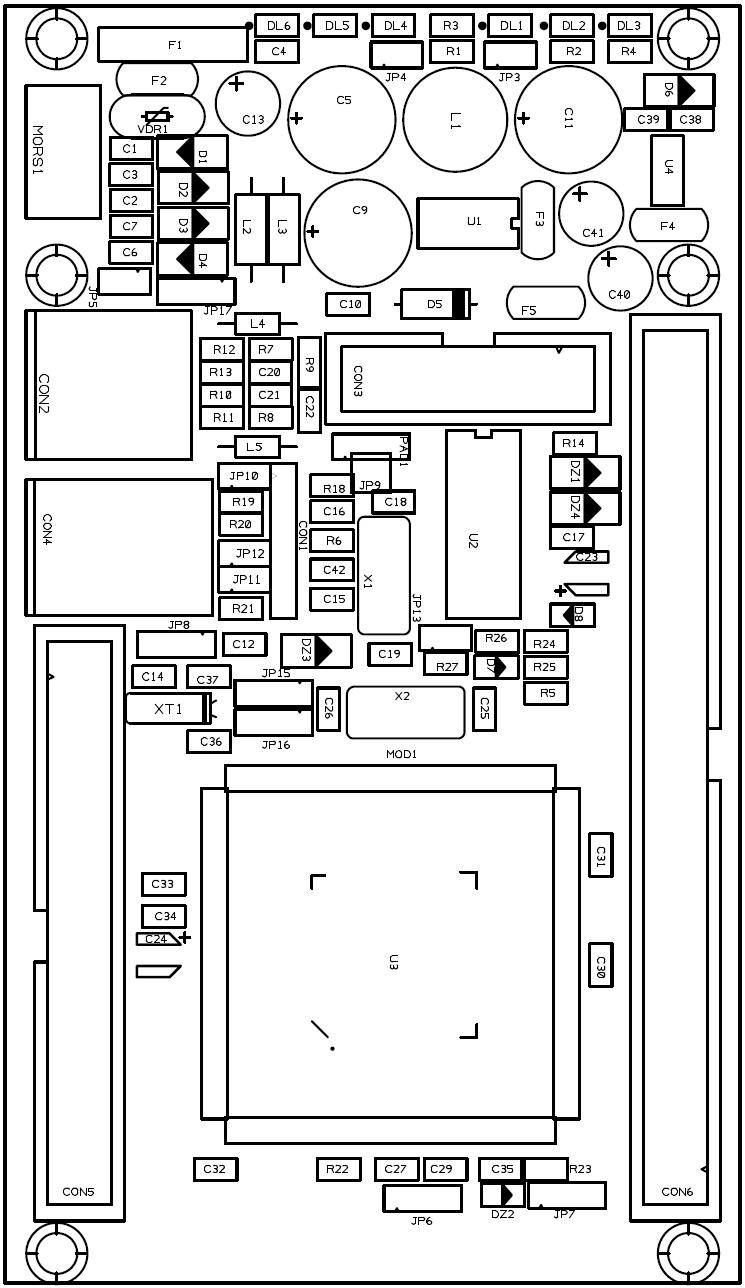
\includegraphics[
  width=12cm, bb=0 0 745 1288]{images/flex_full_PCB.jpg}\end{center}
\caption{Circuito stampato (PCB) della scheda base \flex\ versione Full.}
\label{fig:flex-full-PCB}
\end{figure}

I jumpers disponibili sulla scheda \flex\ sono elencati nella Tabella
\ref{tab:jumpers-full}.

\begin{table}
\begin{centering}\begin{tabular}{|l|l|}
\hline 
Jumper & Funzione \tabularnewline
\hline \hline 
JP3 & Abilita i led per il monitoraggio dell'alimentazione \tabularnewline
\hline 
JP4 & Abilita il led controllato dal \dspic \tabularnewline
\hline 
JP5 & Selettore del GND o PE logico \tabularnewline
\hline 
JP6 & Selettore dell'alimentazione esterna per A/Ds (3.3 V) \tabularnewline
\hline
JP7 & Selettore dell'alimentazione esterna per A/Ds (0 V) \tabularnewline
\hline
JP8 & Selettore del voltaggio di riferimento per il connettore di
programmazione ICSP
\tabularnewline
\hline
JP9 & Selettore dell'alimentazione del processore PIC18 \tabularnewline
\hline
JP10 & Switch del segnale Master Clear tra \dspic\ e PIC18 
\tabularnewline
\hline
JP11 & Switch della linea dati tra \dspic\ e PIC18
\tabularnewline
\hline
JP12 & Switch della linea di programmazione tra \dspic\ e PIC18
\tabularnewline
\hline
JP13 & Resistenza di pull-up opzionale per la porta seriale RX \tabularnewline
\hline
JP15, JP16 & Real-time clock esterno \tabularnewline
\hline
JP17 & Selettore per lo schermo USB verso GND o PE \tabularnewline
\hline
\end{tabular}\par\end{centering}
\caption{Jumper di configurazione disponibili per la scheda \flex\
versione Full.}
\label{tab:jumpers-full}
\end{table}

\begin{itemize}
\item JP3: permette di abilitare i led di monitoraggio
  dell'alimentazione a 5V e 3,3V prima del circuito di switching;
% siamo sicuri che sia prima? non dovrebbero essere a valle?
\item JP4: abilita il led controllato dal microcontrollore \dspic;
\item JP5: permette di connettere il GND logico verso PE;
\item JP6: permette di utilizzare una alimentazione esterna invece
  della alimentazione interna a 3,3 V per il voltaggio positivo degli
  A/D converters del \dspic;
\item JP7: permette di utilizzare una alimentazione esterna invece di
  quella interna a 0 V per il voltaggio negativo degli A/D converters
  del \dspic;
\item JP8: permette di cambiare il voltaggio di riferimento sul
  connettore ICSP fornito dal debugger ICD2 tra 5 V e 3.3 V;
\item JP9: permette di cambiare l'alimentazione del PIC18 tra il
  voltaggio intreno a +5 V e la linea di alimentazione USB;
\item JP10: redireziona il segnale Master Clear proveniente dal connettore
  di programmazione ICSP al microcontrollore \dspic\ o PIC18;
\item JP11: redireziona il segnale di programmazione proveniente dal
  connettore di programmazione ICSP al microcontrollore \dspic\ o
  PIC18;
\item JP12: redireziona il segnale di clock proveniente dal connettore
  di programmazione ICSP al microcontrollore \dspic\ o PIC18;
\item JP13: connette il resistore di pull-up alla linea seriale RX; se
  inutilizzato, il pin � utilizzato come un normale pin GPIO;
\item JP15 and JP16: permette di utilizzare un clock esterno per il
  microcontrollore \dspic; se disabilitati, i due pin possono essere
  utilizzati come normali pin GPIO;
\item JP17: permette di modificare lo schermo USB tra GND o PE.
\end{itemize}

%-----------------------------------------------------------------
\subsection{Scheda base: versione Light}
\label{sec:base-light}
%-----------------------------------------------------------------

La scheda \flex\ versione Light, visualizzata in Figura
\ref{fig:flex-light}, � stata disegnata con l'obiettivo di mantenere
una dimensione la pi� compatta possibile. In particolare, la versione
Light utilizza un circuito di alimentazione semplificato, e pertanto
richiede una alimentazione in generale pi� stabile della versione
Full, come ad esempio quella fornita da una batteria. Inoltre, la
versione Light non possiede il supporto USB. Esempi di applicazioni
che utilizzano la scheda Flex Light sono applicazioni distribuite
alimentate a batteria, come reti di sensori, piccole applicazioni
robotiche, acquisizioni di dati da sensori, ecc...

L'alimentazione della versione Light delle schede base \flex\ deve
essere nel range 9 - 12 V.

\begin{figure}[htb]
\begin{center}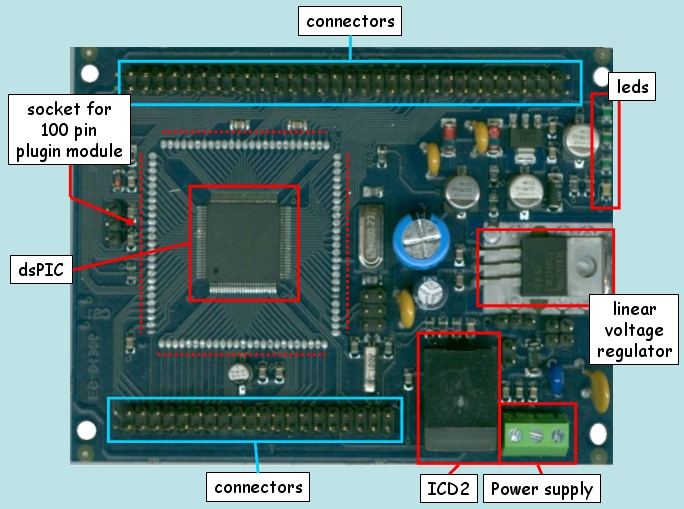
\includegraphics[
  width=12cm, bb=0 0 684 509]{images/flex_base_light.jpg}\end{center}
\caption{La scheda base \flex\ in versione Light.}
\label{fig:flex-light}
\end{figure}

I jumper disponibili nella versione Light sono elencati nella Tabella
\ref{tab:jumpers-light}.

\begin{table}
\begin{centering}\begin{tabular}{|l|l|}
\hline 
Jumper & Funzione \tabularnewline
\hline \hline 
JP3 & Abilita i led per il monitoraggio dell'alimentazione \tabularnewline
\hline 
JP4 & Abilita il led controllato dal \dspic \tabularnewline
\hline 
JP5 & Selettore del GND o PE logico \tabularnewline
\hline 
JP6 & Selettore dell'alimentazione esterna per A/Ds (3.3 V) \tabularnewline
\hline
JP7 & Selettore dell'alimentazione esterna per A/Ds (0 V) \tabularnewline
\hline
JP8 & Selettore del voltaggio di riferimento per il connettore di
programmazione ICSP
\tabularnewline
\hline
JP15, JP16 & Real-time clock esterno \tabularnewline
\hline
\end{tabular}\par\end{centering}
\caption{Jumper di configurazione disponibili per la scheda \flex\
versione Light.}
\label{tab:jumpers-light}
\end{table}

\begin{itemize}
\item JP3: permette di abilitare i led di monitoraggio
  dell'alimentazione a 5 V e 3,3 V prima del circuito di switching;
% siamo sicuri che sia prima? non dovrebbero essere a valle?
\item JP4: abilita il led controllato dal microcontrollore \dspic;
\item JP5: permette di connettere il GND logico verso PE;
\item JP6: permette di utilizzare una alimentazione esterna invece
  della alimentazione interna a 3,3 V per il voltaggio positivo degli
  A/D converters del \dspic;
\item JP7: permette di utilizzare una alimentazione esterna invece di
  quella interna a 0 V per il voltaggio negativo degli A/D converters
  del \dspic;
\item JP8: permette di cambiare il voltaggio di riferimento sul
  connettore ICSP fornito dal debugger ICD2 tra 5 V e 3.3 V;
\item JP15 and JP16: permette di utilizzare un clock esterno per il
  microcontrollore \dspic; se disabilitati, i due pin possono essere
  utilizzati come normali pin GPIO;
\end{itemize}

\begin{figure}[htb]
\begin{center}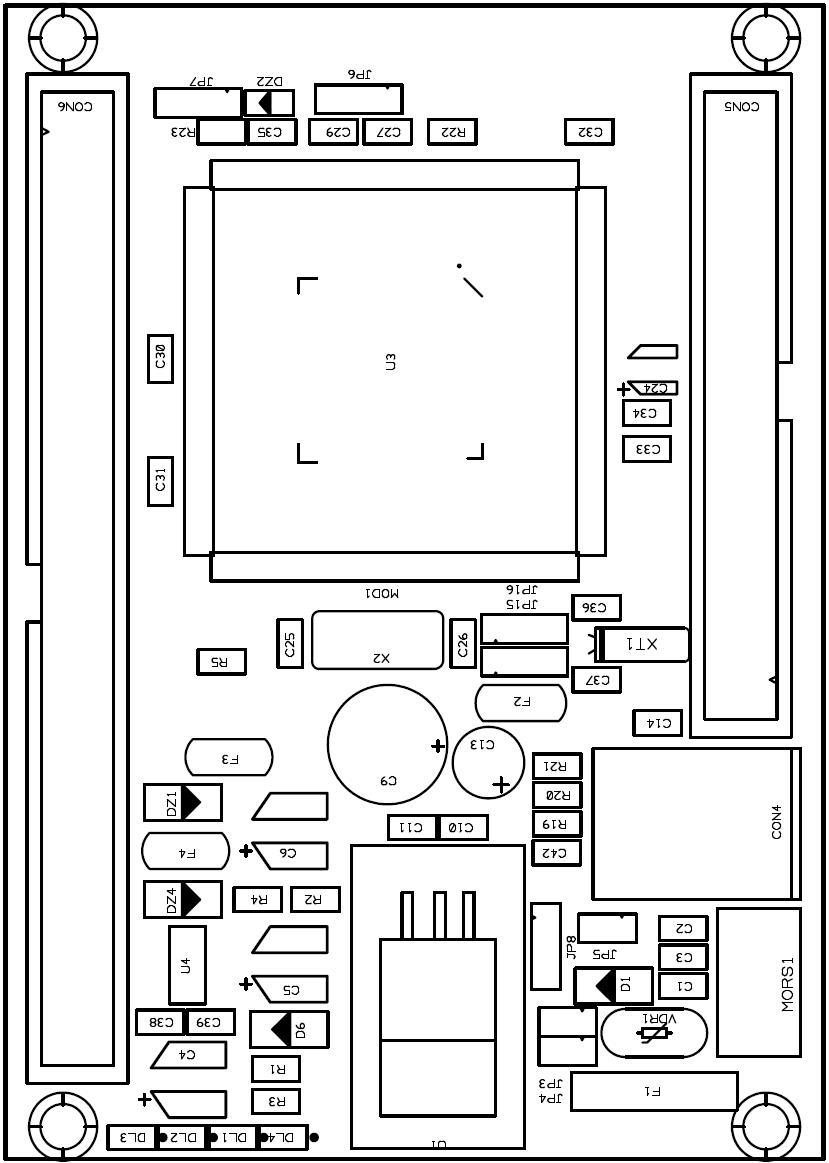
\includegraphics[
  width=12cm, bb=0 0 829 1163]{images/flex_light_PCB.jpg}\end{center}
\caption{Circuito stampato (PCB) della scheda base \flex\ versione Light.}
\label{fig:flex-light-PCB}
\end{figure}

%-----------------------------------------------------------------
\section{Schede figlie}
\label{sec:daughter}
%-----------------------------------------------------------------

Una scheda figlia per le board \flex\ � una scheda con un insieme di
funzioni specializzate che possono essere connesse fisicamente sopra
una scheda base (in ``piggybacking'') per ottenere in generale delle
funzionalit� utili per applicazioni specifiche.

Evidence S.r.l. e Embedded Solutions S.r.l. propongono un insieme di
schede di utilizzo generale per le applicazioni pi� comuni.

Lo sviluppo ``in casa'' di schede figlie � molto semplice, in quanto i
connettori della scheda base utilizzano il passo standard a 2,54
mm. Per questo motivo, le funzionalit� delle schede \flex\ possono
essere estese a piacere senza particolari limiti.


%-----------------------------------------------------------------
\subsection{Scheda figlia millefori}
\label{sec:thru_hole_board}
%-----------------------------------------------------------------

La scheda visualizzata in Figura \ref{fig:thru-hole-board} �
indirizzata per lo sviluppo di piccoli circuiti sviluppati ``in casa''
con l'obiettivo di essere interfacciati in modo semplice con le schede
base \flex.

\begin{figure}[htb]
\begin{center}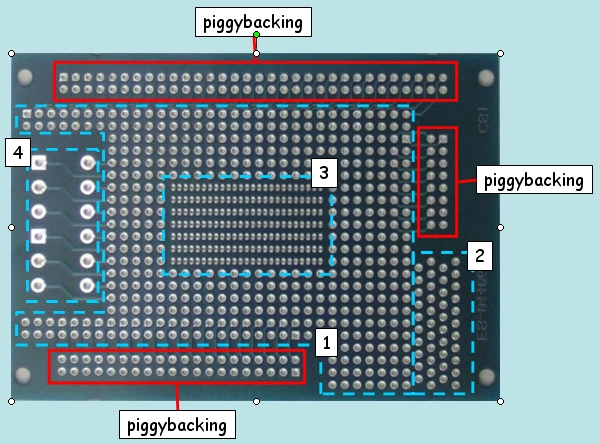
\includegraphics[
  width=12cm, bb=0 0 600 444]{images/thru_hole_board.jpg}\end{center}
\caption{Scheda figlia millefori.}
\label{fig:thru-hole-board}
\end{figure}

La scheda millefori espone diverse tipologie di forature che possono
essere utilizzate per connettere i componenti pi� comuni.

I pattern marcati nella figura con il termine ``piggybacking'' sono
pin che provengono dai connettori della scheda base \flex. Come
visualizzato nella Figura \ref{fig:thru-hole-board}, ogni pin nella
zona dei connettori � connesso verso un pin nella zona centrale della
scheda.

La restante parte dello spazio � diviso nelle tipologie di forature
pi� comuni, come:

\begin{enumerate}
\item pattern standard a 2,54 mm;
\item pattern standard a 2,54 mm con linee alternate, utile per
  connettori RJ45 e RS232;
\item pattern standard a 1,27 mm, utile per saldare dispositivi SMD;
\item pattern standard a 5,08 mm, utile per saldare morsetti;
\end{enumerate}

%-----------------------------------------------------------------
\chapter{Schede figlie personalizzate}
\label{ch:customizations}
%-----------------------------------------------------------------

Esistono una serie di estensioni possibili che possono essere aggiunte
alle schede \flex\ per aggiungere nuove funzionalit�, sensori,
connessioni di rete, attuatori ecc... Le estensioni pi� semplici
possono essere effettuate utilizzando una scheda figlia millefori.

Purtroppo, molte estensioni di \flex\ possono richiedere della
esperienza che pu� richiedere componenti speciali disponibili solo con
montaggio SMD, componenti che difficilmente sono saldabili ``a mano''.

Per evitare il problema, Embedded Solutions Srl � disponibile a
coprire specifiche necessit� di personalizzazione che possono portare
alla produzione di schede figlie per applicazioni particolari. A
seconda del numero di pezzi da produrre, una reingegnerizzazione
dell'intero sistema potrebbe in generale portare a riduzioni di
dimensioni, peso, consumi e costo. Per la realizzazione di tali
sistemi, Embedded Solutions ha capacit� di prototipazione e
assemblaggio di schede multilayer in tecnologia SMT e PTH.

Per maggiori informazioni sul design di schede figlie personalizzate,
non esitate a contattarci!



%-----------------------------------------------------------------
\chapter{Sviluppo Sofware con le schede \flex}
\label{ch:ee-flex}
%-----------------------------------------------------------------

Le schede \flex\ sono accompagnate da una ricca dotazione software che
semplifica notevolmente lo sviluppo applicativo.

\section{\ee}
Le schede \flex\ utilizzano di base l'ambiente di sviluppo \rtd\ ed il
kernel real-time \ee\. In particolare, \rtd\ include lo stato
dell'arte per il design e l'ottimizzazione di una applicazione
real-time, ed il kernel \ee\ fornisce un kernel real-time minimale che
fornisce interessanti feature per il microcontrollore \dspic\ a bordo
di \flex.

\section{Librerie per \flex}
\ee\ supporta le periferiche delle schede \flex\ e delle sue
schede figlie tramite delle apposite librerie. In particolare, le
librerie sono state realizzate in modo tale da accedere in modo
semplice alle varie caratteristiche della scheda base e delle schede
figlie.

Le librerie possono essere configurate utilizzando l'ambiente \rtd,
che semplifica la realizzazione di applicazioni per il
microcontrollore \dspic\ tramite una configurazione grafica ed il
supporto diretto per le librerie all'interno del linguaggio OIL.

\section{Applicazioni di esempio}
Sono disponibili varie applicazioni di esempio che utilizzano la
\flex\ board. Gli esempi sono disponibili come ``template''
all'interno di \rtd, e possono essere selezionati al momento della
creazione di un progetto di \rtd.

\section{Scilab and Scicos code generator}
Infine, � disponibile un generatore di codice capace di generare una
applicazione di controllo digitale a partire da un diagramma
funzionale Scicos. Il generatore di codice per Scicos � stato
sviluppato in collaborazione con Smone Mannori di INRIA (FR)
\cite{scicos}, e Roberto Bucher del SUPSI Lugano
\cite{bucher}. L'ultima versione del generatore e della relativa
documentazione � disponibile sul sito web Evidence
\url{http://www.evidence.eu.com}.

%-----------------------------------------------------------------
\chapter{Dove acquistare le schede \flex}
\label{ch:howtobuy}
%-----------------------------------------------------------------

Le schede \flex\ possono essere acquistate attraverso i seguenti
distributori:


\subsection{Italia}


\includegraphics[width=3cm, bb=0 0 145 60]{images/elettroshop.jpg}

\noindent Link verso il sito di e-commerce:
\begin{itemize}
\item Scheda \flex versione Full -
  \url{http://www.elettroshop.it/dettagli.asp?pid=1352}
\item Scheda \flex versione Light -
  \url{http://www.elettroshop.it/dettagli.asp?pid=1355}
\end{itemize}

\noindent {\bf Inware S.r.l.}\\
Via Cadorna, 27/31 \\
20032 Cormano (MI) \\
Tel: +39 02 66504794 \\
Fax: +39 02 66508225 \\
URL: \url{http://www.inware.it/} \\
Email: info[at]inware.it \\

\subsection{Stiamo cercando distributori!}

Non esitate a contattarci se siete un distributore e volete
distribuire \flex\ in altri Stati!
